\chapter{Learning speech acts}
\label{chap:eng-sp}

As we have discussed in the last three chapters, pragmatics is crucial for children to learn clause type categories, and even noisy pragmatics can benefit the learner. But then, there still remains the question of how children learn speech act categories? Given that the way we generally identify a speech act is via its clause type, there is a potentially vicious circle here: you need to know the clause type to identify the speech act, but you need to know the speech act to identify the clause type. %How do learners avoid this circularity? 

But as we have discussed in Chapter~\ref{chap:introduction}, it is likely that children learn to identify speech act and clause type in tandem and mutually informative ways: children learn to identify clause types by tracking morpho-syntactic and prosodic regularities in conjunction with their growing
knowledge of speech act and its associated behavioral cues; similarly, they learn
to identify speech acts by tracking social pragmatic cues and prosodic cues in conjunction with their growing
understanding of the formal features of various clause types.


In the last two chapters, we have already seen that even if children have limited access to the speech act information, they might still benefit from it when learning to cluster clause types. If children do not need \emph{perfect} speech act information to figure out clause types, then we do not need to assume that by the time children are learning to figure out clause types, they have already figured out speech acts. 

But what about the learning of speech act categories? Even if children must rely on clause type information to figure out the speech acts, they could have access to additional information that is unrelated to clause typing, but informative for recognizing speech act type. For example, in conversations, we use questions to elicit responses and information, which leads to behaviors like pausing after questions, or looking directly at our interlocutor, to nudge them to answer our questions. We also tend to use rising contours to perform questions, as discussed in Chapter~\ref{sec:bg:theory:prosody}.
This in turn means that we can expect different kinds of behavior to be correlated with these acts. So, armed with an innate category for questions, and a theory of what questions do in conversations, the child can expect certain kinds of nonlinguistic behavior to be correlated with the act of asking a question. If these behavior are also correlated with the act of asking a question in the input, then they can tell whether their parent is asking them a question.  

But just as surface features might be absent or misleading in the input, the social pragmatic features and prosodic features might also be absent or misleading. Therefore, I ask in this chapter whether it is possible to see some social pragmatic and prosodic features correlated with speech acts. I focus on the questioning act here, as this speech act is relatively well understood, and plan to extend to requests/commands in the future.

So what do we do when we ask questions? First, 
as we have discussed in Chapter~\ref{chap:prosody} pitch rises tend to signal questions and pitch falls signal assertions; and some argue that this universality reflects the innate knowledge that high rising pitch connects to the speech act of questioning (\cite{ohala1984,gussenhovenchen2000,gussenhoven2002} among others). If children are armed with this knowledge that questions are associated with rising contours, they might expect rising contours to be correlated with the act of asking a question. If the input is such that more questions are uttered with rising contour than assertions, then this could be helpful for the child to figure out what utterances are  questions in their input. But just as not all interrogatives have subject-auxiliary inversion and not subject-aux inversion are interrogatives, not all questions have final rises (\cite{gussenhoven2000fallq, hedberg2004wh,ladd2008intonational}), and not all final rises are questions (e.g. \cite{gordon1999prosody,ladd1981, ward1985rfr,goodhue2016prosody}). In English, \twh-questions are usually produced with final fall (\cite{hedberg2004wh,ladd2008intonational}), and the rise-fall-rise contour could be associated with assertions (\cite{ladd1981, ward1985rfr,goodhue2016prosody}). Nevertheless, it is still possible that more questions than assertions are produced with rises in the input, which could still be informative for the child. We therefore need to verify empirically whether prosodic information is potentially informative.


Questions are also devices for us engage with an addressee. When we ask questions, we are looking for information, or sometimes simply for a response. This makes questions perfect turn-transition points (\cite{duncan1972turn} among many others), signaling that the current speaker is done with the turn and the next speaker needs to get ready. This makes the use of questions to be correlated with  communicative signals like direct eye gaze: speakers gaze at their interlocutor longer after questions (\cite{argyle1972gaze}). When we are looking at our interlocutor for an answer, we might have certain facial expressions. For example, \textcite{domaneschi2017facial} find people tend to associated with the facial expressions pictured in Figure~\ref{fig:engsp:au} with questions. If children are equipped with the knowledge about facial expressions, they might be able to exploit the correlation between questioning and facial expressions to learn about questions. 
\begin{figure}[H]
    \centering
    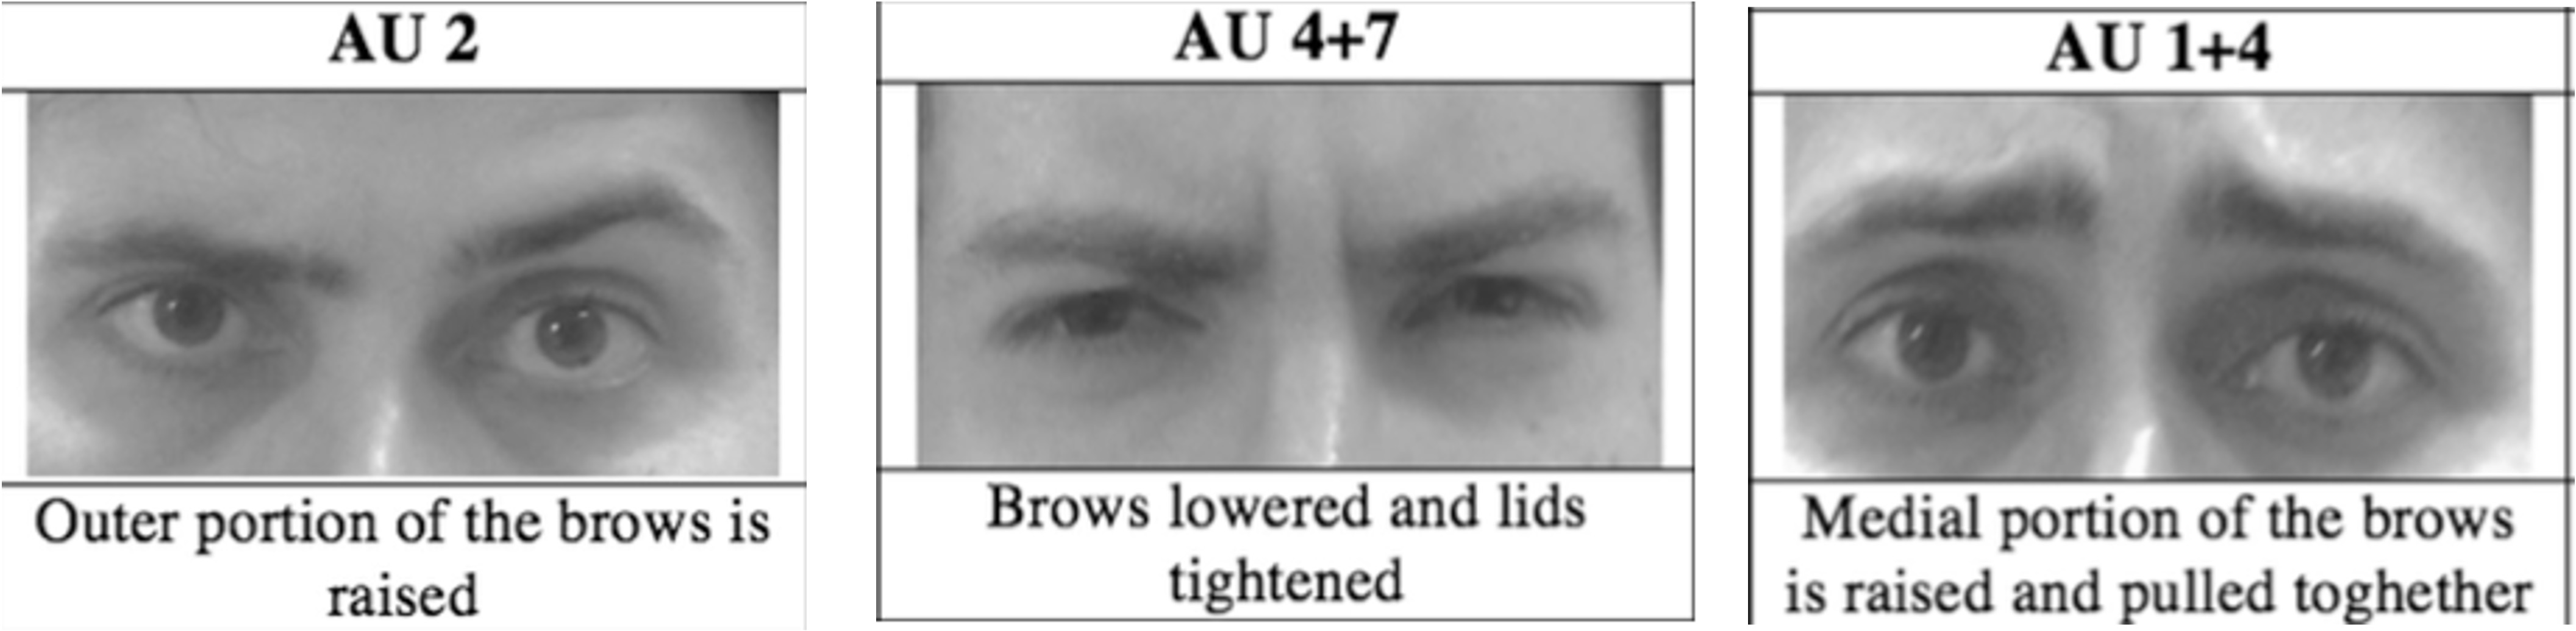
\includegraphics[width=1\textwidth]{figures/q-aus.jpg}     
    \caption{The upper face action units (AU) identified by participants as indicating the act of questioning, as reported by \cite{domaneschi2017facial}}
    \label{fig:engsp:au}
\end{figure}

Another similar conversational signal might be the time in-between conversational turns. A property related to a turn-transition point is that interlocutors use these points as cues for when to take over the turn. In a natural face-to-face conversation, the gap between a question and its answer might be smaller than other pairs of utterances in a conversation (\citealt{tice2011turn} a.o.). But the questioner might also pause and wait if nobody steps in immediately (\cite{sacks1978pause}). Therefore, tracking the gap after utterances might tell us whether the utterance is a question.


So if children understand the mechanism of human communication, which as we have in Chapter~\ref{chap:background} that they do, and have the prior knowledge that certain speech acts expects responses, they might expect to see a correlation between questions and the length of eye gaze, the facial expressions of their interlocutor, and the length of pauses. They then can exploit this correlation to learn questions.

We express our desire to know with questions (e.g.\cite{searle1975tax, krifka2011q, carruthers2018q}). As a result, when we ask questions, we might be ignorant of certain information. If children can keep track of who knows what, and as we saw in Chapter~\ref{chap:background} that they can, they can exploit this correlation between lack of information with questions to infer questionhood. However, this correlation might not show up in the input, as parents tend to use questions as a tool for teaching. A parent asking ``What's that?'' is likely not to solicit some information they don't know, but to see if the child knows it too. Previous corpus study suggests that about 38\% of parents' questions when the child is before 2 years old are pedagogical questions (\cite{yu2019pedagogical}), and for middle class parents, this number could reach 60\%. The child might still be able to exploit the cue in some way, but it might not be as straightforward.  

Due to the limitation of our corpus data, in this chapter we will examine the following features: prosody, duration of pauses between utterances, and eye gaze. This chapter is organized as follows: Section~\ref{sec:engsp:background} reviews previous evidence for children's perception of these cues. I then report results from a corpus study with Providence Corpus in Section~\ref{sec:engsp:corpus}, where I looked at the prosody of parents' utterances (Section~\ref{sec:engsp:results:prosody}), pauses between parents' utterances (Section~\ref{sec:engsp:results:pause}), and parents' attentional behavior (\ref{sec:engsp:results:gaze}).
Section~\ref{sec:engsp:discussion} concludes the chapter.


\section{Background}
\label{sec:engsp:background}
\subsection{Pauses in conversation}
\label{sec:engsp:bg:pause}
As mentioned earlier, questions are turn-transition points (\cite{duncan1972turn} among others), and this means that speakers anticipate a change of turn after questions. In adult-to-adult conversations, this property translates to shorter speech gaps after questions in one-on-one in-person conversations (\cite{stivers2010,enfield2010,hilbrink2013turn} among many others). Speakers might also wait after questions for responses (\cite{sacks1978pause}), but for adults, longer inter-turn silence leads to feelings of unease and tend to be avoided (\cite{roberts2006pause} among others). But when interacting with pre-linguistic infants, this silence might be helpful rather than awkward: if children can track the length of pause after an utterance, they might be able to infer that longer pauses are associated with questions and request. Are children sensitive to the turn-taking properties of conversations? 
%As infants could use prosodic cues to detect clause boundaries (\cite{hirsh1987clause, seidl2007prosody}), they might be able to track the length of pause after an utterance. 

As early as 3 months old, infants show sensitivity to the structure of conversation. The overlap between infant vocalization and parents' speech decreases overtime, and the average gap between parent utterance and infant vocalization decreases, suggesting that they respect the turn-taking rules (\cite{hilbrink2013turn3mo}). When they start producing one-word utterances, slow down at trying to change turn, but quickly pick up the speed again as their linguistic ability develops (\cite{hilbrink2013turn}).

Studies also show that same as adults, children interpret pauses as meaningful. \textcite{craiggallagher1983pause} 
investigate whether or not 22-36-month-olds abandon their request (e.g. wanting a cookie) after the parent's initial responses (classified as neutral, e.g. \tit{you want what?},  negative, \tit{No.} or pause). They found that the older children (3-year-olds) abandon requests after adult pauses for more than 1s, suggesting that children treat long pauses as a meaningful response. This is suggestive, but based on this research alone it remains unclear whether children associate inter-turn silence with the interlocutor trying to elicit a response. 

%Bloom et al: four children, 21 to 36 months of age. Adjacent speech is more than anything from the beginning, Contingent speech increase over time (adjacent (immediately preceded by an adult utterance), or as nonadjacent (not immediately preceded by an adult utterance). Adjacent utterances were either contingent (shared the same topic and added new information relative to the topic of the prior utterance), imitative (shared the same topic but did not add new information), or noncontingent (did not share the same topic). Linguistically contingent speech (speech that expanded the verb relation of the prior adult utterance with added or replaced constituents within a clause)  occurred more often after questions than nonquestions. 

On the other side the problem, the length of pauses results from the dynamics of conversation; if parents are interacting with a pre-linguistic infant, would they follow the same rules? In other words, if we assume that children can keep track of the length of pauses, are there any patterns found in the silences? Previous studies show that parents seem to treat even pre-linguistic infants as competent conversationalists, and any vocalizations (e.g. crying, babbling) or even body movements, are treated as a conversational turn (\cite{beebe1988,jaffe2001turn}). The length of pauses also correlates with the vocabulary of children (\cite{marklund2015pause}). Different from adult-to-adult interactions, parents of 14-month-olds tend to follow questions with another question (\cite{reimchen2017}).  

While these studies show that parents respect turn-taking rules when interacting with pre-verbal infants, little is known about whether parents' speech gaps are informative of the speech act performed. To address this problem, Section~\ref{sec:engsp:results:pause} examines the correlation between the speech act of an utterance and the length of pauses after an utterance, to see if the gap between utterances is informative of an utterance's speech acts. 

\subsection{Attentional behavior}
\label{sec:engsp:bg:gaze}

Another consequence of the response-expectation property of questions is that by the end of a question, the speaker tends to appoint the next speaker. A common device for turn allocation is eye gaze (\citealt{argyle1972gaze, kendon1967gaze,duncan1979gaze, rossano2009gaze, csibra2010}). In dyadic interactions, we tend to look at our interlocutor when we need their response. Thus, it is possible that by tracking where the parent attends to, specifically whether the parent is directly looking at the learner, the learner might be able to infer whether a question is being asked. 

We have seen in Chapter~\ref{sec:bg:acq:pre} that infants are sensitive to the direction of eye gaze since birth. 3-day-old newborns prefer to look at the face that appears to make eye contact with them, suggesting that they are sensitive to the position of the pupils/irises within the eye (\cite{farroni2004gaze}).


While these studies show that infants can perceive parents' direction of eye gaze, and that adults use eye gaze for turn allocation, so far little is known about whether parents' gaze pattern correlates with turn allocation, and furthermore, with the speech act of an utterance. If questions signals a transition of turn, parents' gaze should fall on the addressee--the child--more after questions. I address this question in Section~\ref{sec:engsp:results:pause} by examining parents gaze pattern during parent-child interactions, to see if this cue is informative of an utterance's speech acts.

\subsection{Interim Summary}
\label{sec:engsp:bg:summary}

When interacting with other people, we use many cues, besides the clause type information, to infer what kind of speech act is being performed. In particular, since questions usually signal the transition of a conversational turn, the questioner usually shifts gaze to the next designated speaker. Adults can also infer from a question being performed that the questioner wants someone to pick up the turn, and thus the lengths of speech gap after questions are normally longer than lengths of pause after other speech acts. However, if we look at dyadic interactions between a parent and a child, especially a child as young as 18 months old, these cues might not show up, or show up in a different way. We should ask, for example, whether parents in child-directed interaction also use direct eye gaze to indicate the next speaker, i.e. the child? Also, since 18-month-olds are not mature conversationalists, the speech gap after utterances might be longer across the board, so are there any differences in pauses that correlate with the speech act being performed? Another potential cue is prosody. In English, yes/no questions are usually associated with a special final rise contour (L* H-H\%), which can be produced with either polar interrogatives and declaratives syntax. Would final rises be a cue that distinguishes between the three speech acts?

To address these questions, we built a multi-modal dataset with dyadic parent-child interactions for infants before 18 months old, to see if there is any non-clause type cues that may help infants distinguish speech acts.

\section{Corpus study}
\label{sec:engsp:corpus}

This section details the corpus study we conducted to investigate whether speech gap, direct gaze, and prosody in dyadic parent-child interactions correlate with parents' use of different speech acts. 


\subsection{Methods}
\label{sec:engsp:corpus:method}
This study also used data from the Providence Corpus (\citealt{ProvidenceCorpus}) from CHILDES system (\citealt{CHILDES}). The audio and video of the sessions sampled in Chapter~\ref{chap:eng-cl} and Chapter~\ref{chap:prosody} were extracted for annotation. 


For annotating gaze, we used the video data available in the Providence corpus. Trained annotators viewed the muted videos using ELAN (\cite{elan}). Each video was annotated first with whether the parent and the child are visible on screen and the parent's focus of attention can be identified. If the parent is only half on screen, but we can still identify the focus of attention of the parent, this proportion was counted as on-screen. If the parent is on screen but the focus cannot be identified due to bad lighting, this proportion of the video was counted as off-screen.

Then, for the parts of the video that both the parent and the child are both on screen, the focus of parents' attention was annotated. Specifically, whether the parent is paying attention to the child, to an object, or unidentifiable. The parent was annotated as paying attention to the child when they attended to the child through (1) direct eye gaze (when the eyes could be seen), (2) head or body orientation toward the child (when the eyes could not be seen), (3) physical interaction with the child. I then used a script to calculate the proportion of looks to the child during the utterance, and at 1s, 2s, 3s before and after the utterance.%, by dividing the total length of the on-screen time by the length that the parent attends to the child.  
 
\subsection{The correlations we expect}
\label{sec:engsp:predictions}
If speech gaps and gaze are indeed useful cues to obtain speech act information, we would expect the following predictions to bear out.


For speech gaps, we should see that parents pause longer after questions and requests than after assertions, to wait for responses.
And for eye gaze, we should see that parents direct attention to the child more often after questions and requests than after assertions. 


\subsection{Results}
\label{sec:engsp:results}

\subsubsection{Pauses}
\label{sec:engsp:results:pause}

For this cue, we measured the length of silence between parents’ consecutive utterances like (\ref{code-prag:pause}). To do so, we first followed the methodology of \textcite{bloom1976discourse} and annotated for each utterance whether it is a contingent utterance of the previous one, i.e.\ whether it shares the same topic and adds new information relative to the topic of the prior utterance. We will refer to such pairs of utterances, with one contingent on the previous utterance like in (\ref{code-prag:pause}), as consecutive turn sequences. Within the sequences, I measured the length of pauses between utterances. 


\bex{code-prag:pause}
%\bxl{}
\tbf{Consecutive turn sequence}
\bxl
You can’t take your rake on the swing.\\
 \tsc{pause: 0.014s} \\ 
 You wanna take your big bird rake on the swing? 			\hfill \tsc{Assertion -Question}
\ex You don't wanna swing?\\
 \tsc{pause: pause: 0.23s} \\	
 You don’t have to.	\hfill \tsc{Question-Assertion}
\ex Here you use this one. \\
 \tsc{pause:  0.033s} \\ This one works better.	\hfill \tsc{Assertion-Assertion}
\exl
\eex

In total, 4066 utterances were found to have a contingent follow-up that allows us to measure the inter-turn silence. Figure~\ref{fig:engsp:pause} shows the length of pause after each speech act category.

\begin{figure}[H]
\begin{center}
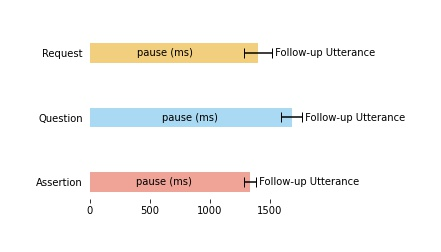
\includegraphics[width = 0.8\textwidth]{figures/pause.jpg}
	\caption{Duration of pause (ms) after each type of speech act}\label{fig:engsp:pause}
\end{center}
\end{figure}

These results show that parents are equally likely to ask another question as they are to answer their own questions, but parents tend to pause longer after questions (mean $= 1728ms$) than assertions (mean $= 1321ms; t(2925) = -2.23, p = 0.02$), suggesting that parents pause after asking a question but proceed with the conversation after an assertion. %There is no difference between questions and requests mean $= 1345ms; t(1418) = 0.83, p = 0.4$), suggesting

\begin{comment}
\begin{figure}[H]
\begin{center}
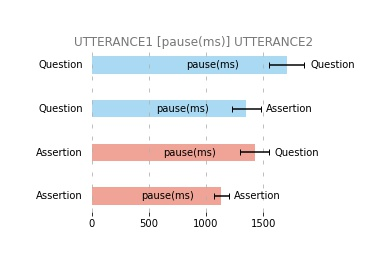
\includegraphics[width = 0.8\textwidth]{figures/pause-QA.jpg}
	\caption{Duration of pause (ms) between Question-Question/Assertion and Assertion-Question/Assertion pairs }\label{fig:engsp:pause-QA}
\end{center}
\end{figure}
\end{comment}


\subsubsection{Parents' attentional behavior}
\label{sec:engsp:results:gaze}

In total, 857 utterances were found to have attentional data suitable for annotation. Figure~\ref{fig:attention} shows the proportion of looks to the child before, during, and after an utterance.


\begin{figure}[H]

\begin{center}
	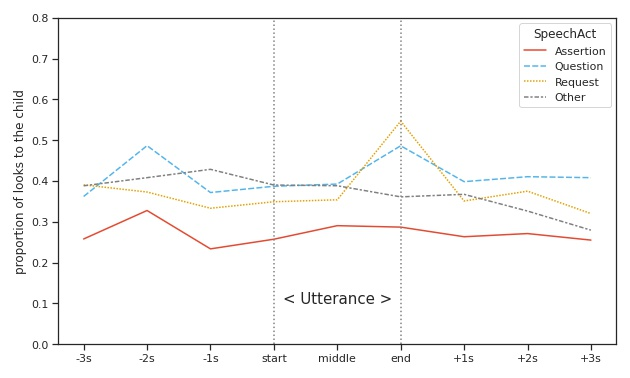
\includegraphics[width =1\textwidth]{figures/gaze-pattern-adult.jpg}
	\caption{Proportion of parents' looks to the child before, during, and after an utterance} \label{fig:attention}
\end{center}
\end{figure}


From Fig.~\ref{fig:attention}, we can see that when the utterance is a question, the proportion of looks to the child is higher (average $0.41$) than when it is an assertion (average $0.27; t(16) = 2.53, p <0.05$), but roughly equivalent to when the utterance is a request ($0.37; t(16)= 1.27, p=0.21$). These results suggest that parents look at the child longer after questions and requests. %%%%; in the post-utterance region, the proportion of looks to the child is higher when the utterance is a question ($0.53$) than when it is an assertion ($0.25; t(4) = 7.95, p<0.05$) but not when it's a request ($0.39; t(4) = 4.2, p=0.2$). 

\begin{comment}


\subsubsection{Informativeness of the cues}
\label{sec:engsp:results:stats}
A multinomial logistic regression model was built with the three cues as independent variables, and the speech act categories (assertions, questions, requests, and other) as the dependent variable. The data for the model was an intersection of the prosody, pause, and attentional data, as not all utterances have follow-up utterances for us to measure the inter-turn silence, and some utterances were uttered off screen with no attentional data. In total, 806 utterances were included in the analysis.  We then split the data into a training set (90\% of the data) and testing set (10\%), and trained a logistic regression classifier with the training data. For details of the model, see Appendix~\ref{appx}. This classifier can predict 57\% of the speech act labels, suggesting that the three cues could to some extend help children identify speech act information. 
\end{comment}

\section{Conclusion}
\label{sec:engsp:discussion}
In this chapter, we turn to the problem of speech acts, specifically how parents use questions in their interaction with children. As questions are often used to elicit responses and information, we can expect different kinds of behavior to be correlated with these acts. Armed with an innate category for questions, and a theory of what questions do in conversations, the child can expect certain kinds of non-clause type cues to be somewhat correlated with the act of asking a question. 

Some candidates for cues that could potentially differentiate questions from other speech acts are pauses and direct eye gaze. The canonical function of questions is to solicit responses or seek information, so when we use questions, it is likely that we pause after questions, or look directly at our interlocutor, as a way to signal to them that they need to take over the conversational turn. As we have reviewed, children have a theory of communication early on, and understand the structure of conversations from as young as three months old (\cite{casillas2016corpus}). With this theory of communication, and the prior knowledge that certain speech act is used for response-elicitation, they may expect questions to be correlated to some degree with longer pauses and direct eye gaze. I found that these features are correlated with the act of questioning in the input: parents tend to pause longer after questions, and attend the child more when asking questions. To the extent that they are weakly correlated with the questioning act, it is in principle plausible that (a) a child could use these features, in addition to their growing knowledge of clause types to infer the speech act category of an utterance; and (b) this little bit of information about speech act could then be used to provide the 20\% of pragmatic information that the child needs in order to get the clause type clusters identified accurately.


